\documentclass{beamer}
\usetheme[numbering=none,progressbar=frametitle]{metropolis}
\usepackage{cmap}%
\usepackage{alphabeta}%
\usepackage[greek,english]{babel}%
\languageattribute{greek}{polutoniko}%
\usepackage{hyperref}%
\usepackage{lmodern}%

\usepackage{xcolor}%
\usepackage{mathtools}%
\usepackage{mdframed}%
\usepackage[inline]{enumitem}%
\usepackage{natbib}%
\usepackage[toc,page]{appendix}%
\usepackage{stmaryrd}%
\usepackage{comment}%
\usepackage{ifthen}%
\usepackage{tikz}%
\usepackage{tikz-qtree}%
\usepackage{tikz-qtree-compat}%

\usepackage{amsmath, amscd, amsthm, amssymb, mathrsfs, amsfonts, wasysym}%
\let\oldemptyset\emptyset%
\let\emptyset\varnothing%

\usepackage{bussproofs}%
\EnableBpAbbreviations%
\def\fCenter {\mathbin{\vdash}}%
\def\la      {\leftarrow}%
\def\ra      {\rightarrow}%
\def\impl    {\mathbin{\slash}}%
\def\impr    {\mathbin{\backslash}}%
\def\prod    {\bullet}%
\def\prodl   {\bullet}%
\def\prodr   {\bullet}%
\def\himpl   {\fatslash\ }%
\def\himpr   {\fatbslash}%
\def\hprod   {\mathbin{\circ}}%
\def\hprodl  {\mathbin{\circ}}%
\def\hprodr  {\mathbin{\circ}}%
\def\unit    {\ensuremath{\mathbf{I}}}%
\def\sq      {\ensuremath{\Box}}%
\def\di      {\ensuremath{\Diamond}}%
\def\diIfx   {\ensuremath{\hat{\di}}}%
\def\sqIfx   {\ensuremath{\hat{\sq}}}%
\def\diExt   {\rotatebox[origin=c]{180}{\diIfx}}%
\def\sqExt   {\rotatebox[origin=c]{180}{\sqIfx}}%
\def\vsep    {\ \vert\ }%
\def\e       {\ensuremath{\mathbf{e}}}%
\def\t       {\ensuremath{\mathbf{t}}}%
\def\lamET   {\ensuremath{\lambda^{\ra}_{\{\e,\t\}}}}%
\def\S       {\text{S}}%
\def\N       {\text{N}}%
\def\NP      {\text{NP}}%
\def\PP      {\text{PP}}%
\def\INF     {\text{INF}}%
\def\A       {\text{A}}%
\def\IV      {\text{IV}}%
\def\TV      {\text{TV}}%
\def\I       {\ensuremath{\mathbf{I}}}%
\def\B       {\ensuremath{\mathbf{B}}}%
\def\C       {\ensuremath{\mathbf{C}}}%
\def\john    {\ensuremath{\text{john}}}%
\def\mary    {\ensuremath{\text{mary}}}%
\def\bill    {\ensuremath{\text{bill}}}%
\def\walks   {\ensuremath{\text{walks}}}%
\def\likes   {\ensuremath{\text{likes}}}%
\def\plug    {\ensuremath{\:\cdot\:[\:\cdot\:]}}%
\def\DEDICATE{\ensuremath{\mathbf{dedicate}}}
\def\PERSON  {\ensuremath{\mathbf{person}}}
\def\AUTHOR  {\ensuremath{\mathbf{author}}}
\def\OCEAN   {\ensuremath{\mathbf{ocean}}}
\def\WROTE   {\ensuremath{\mathbf{wrote}}}
\def\SCARED  {\ensuremath{\mathbf{scared}}}
\def\BOOK    {\ensuremath{\mathbf{book}}}
\def\READ    {\ensuremath{\mathbf{read}}}
\def\LIKE    {\ensuremath{\mathbf{like}}}
\def\FEAR    {\ensuremath{\mathbf{fear}}}
\def\KURT    {\ensuremath{\mathbf{kurt}}}
\def\MARY    {\ensuremath{\mathbf{mary}}}
\def\JOHN    {\ensuremath{\mathbf{john}}}
\def\PEPIJN  {\ensuremath{\mathbf{pepijn}}}
\def\SAY     {\ensuremath{\mathbf{said}}}
\def\OF      {\ensuremath{\mathbf{of}}}


\newcommand{\qr}     [1][{\cdot}]{\mathbf{Q}(#1)}%
\newcommand{\focus}  [1]{\boxed{#1}}%
\newcommand{\struct} [1]{{\cdot}#1{\cdot}}%
\newcommand{\tr}     [1]{\llbracket #1 \rrbracket}%
\newcommand{\trd}    [1][({\cdot})]{#1^{**}}%
\newcommand{\case}   [4]{\text{case}\;#1\;\text{of}\;(#2, #3)\ra#4}%
\newcommand{\add}[2]{#1 + #2}

\renewcommand*{\&}{%
  \relax
  \ifmmode
    \mathbin{\char`\&}%
  \else
    \char`\&\relax
  \fi
}

\newenvironment{pfbox}[1][1.0]%
  {\gdef\scalefactor{#1} \leavevmode\hbox\bgroup}
  {\scalebox{\scalefactor}{\DisplayProof} \egroup}

\usepackage{appendixnumberbeamer}
\def\solp{\bullet}
\def\holp{\circ}
\def\sofs{\slash}
\def\sobs{\backslash}
\def\hofs{\!\!\fatslash}
\def\hobs{\fatbslash\!}
 

\author{Pepijn Kokke}
\title{A bunch of things to do with NL$_{\lambda}$}
\date{December 7$^{ th }$, 2016}

\begin{document}
\maketitle

\begin{frame}
  \frametitle{What is NL$_\lambda$?}
  \centering
  \only<2>{%
    \def\solp{\holp}
    \def\sobs{\hobs}
    \def\sofs{\hofs}}%
  \vspace*{1em}
  \vfill
  \(\!
  \begin{aligned}
    &\text{Formula} &&\; A, B
    &&\coloneqq \only<1>{\alpha}\only<2>{\ldots}
    \mid A \sobs B \mid B \sofs A
    \\
    &\text{Structure}^+ &&\; \Gamma
    &&\coloneqq \only<1>{\struct{A}}\only<2>{\ldots}
    \mid A \solp B
    \\
    &\text{Structure}^- &&\; \Delta
    &&\coloneqq \only<1>{\struct{A}}\only<2>{\ldots}
    \mid A \sobs B \mid B \sofs A
    \only<2>{%
    \\
    &\text{Context} &&\; \Sigma
    &&\coloneqq \square
    \mid \Sigma \prod \Gamma \mid \Gamma \prod \Sigma
    }
  \end{aligned}
  \)
  \vfill
  \only<1>{%
    \begin{pfbox}
      \AXC{}
      \RightLabel{Ax}
      \UIC{$\struct{\alpha} \fCenter \struct{\alpha}$}
    \end{pfbox}
  }
  \only<2>{%
    \vfill
    \begin{pfbox}
      \AXC{$\Sigma[\Gamma] \fCenter \Delta$}
      \doubleLine\RightLabel{$(\lambda)$}
      \UIC{$\Gamma \holp \lambda x.\Sigma[x] \fCenter \Delta$}
    \end{pfbox}
  }
  \vfill
  \begin{pfbox}
    \AXC{$\Gamma\fCenter\struct{A}$}
    \AXC{$\struct{B}\fCenter \Delta$}
    \RightLabel{L$\sobs$}
    \BIC{$\struct{A\sobs B}\fCenter \Gamma\sobs \Delta$}
  \end{pfbox}%
  \begin{pfbox}
    \AXC{$\Gamma \fCenter \struct{A}\sobs\struct{B}$}
    \RightLabel{R$\sobs$}
    \UIC{$\Gamma \fCenter \struct{A \sobs B}$}
  \end{pfbox}
  %\vfill
  %\begin{pfbox}
  %  \AXC{$\Gamma\fCenter\struct{A}$}
  %  \AXC{$\struct{B}\fCenter \Delta$}
  %  \RightLabel{L$\sofs$}
  %  \BIC{$\struct{B\sofs A}\fCenter \Delta\sofs \Gamma$}
  %\end{pfbox}%
  %\begin{pfbox}
  %  \AXC{$\Gamma \fCenter \struct{B}\sofs\struct{A}$}
  %  \RightLabel{R$\sobs$}
  %  \UIC{$\Gamma \fCenter \struct{B \sofs A}$}
  %\end{pfbox}
  \vfill
  \begin{pfbox}
    \AXC{$\Gamma \solp \Gamma' \fCenter \Delta$}
    \doubleLine
    \RightLabel{Res$\solp\sobs$}
    \UIC{$\Gamma \fCenter \Gamma' \sobs \Delta$}
  \end{pfbox}
  %\begin{pfbox}
  %  \AXC{$\Gamma \solp \Gamma' \fCenter \Delta$}
  %  \doubleLine
  %  \RightLabel{Res$\solp\sofs$}
  %  \UIC{$\Gamma' \fCenter \Delta \sofs \Gamma'$}
  %\end{pfbox}  
  \vfill
\end{frame}

\begin{frame}
  \frametitle{So why this $\lambda$ rule?}
  \begin{minipage}{0.4\linewidth}\centering
    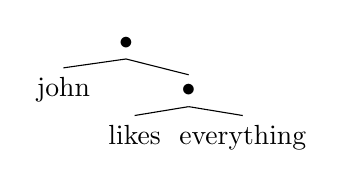
\begin{tikzpicture}
      \tikzset{level distance=4ex}
      \tikzset{sibling distance=0pt}
      \Tree [.$\solp$ john [.$\solp$ likes everything ] ]
    \end{tikzpicture}
  \end{minipage}%
  \begin{minipage}{0.05\linewidth}\centering
    $\longleftrightarrow$
  \end{minipage}%
  \begin{minipage}{0.5\linewidth}\centering
    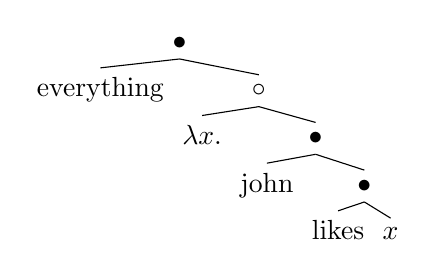
\begin{tikzpicture}
      \tikzset{level distance=4ex}
      \tikzset{sibling distance=0pt}
      \Tree [.$\solp$ everything [.$\holp$
      $\lambda x.$ [.$\solp$ john [.$\solp$ likes $x$ ] ] ] ]
    \end{tikzpicture}
  \end{minipage}
\end{frame}

\begin{frame}
  \frametitle{Why should we like NL$_{\lambda}$?}
  \only<1>{%
    \vfill
    \begin{block}{Example 1}
      ``I read a book [the author of which] feared the ocean''         
      \vfill
      \begin{align*}
        \exists{x}.&\BOOK(x)
        \\
        &{\wedge}\;\FEAR(\iota(\lambda{y}.\OF(y,\AUTHOR,x)),\iota(\OCEAN))
        \\
        &{\wedge}\;\READ(\PEPIJN,x)
      \end{align*}
    \end{block}
    \vfill
  }
  \only<2>{%
    \centering
    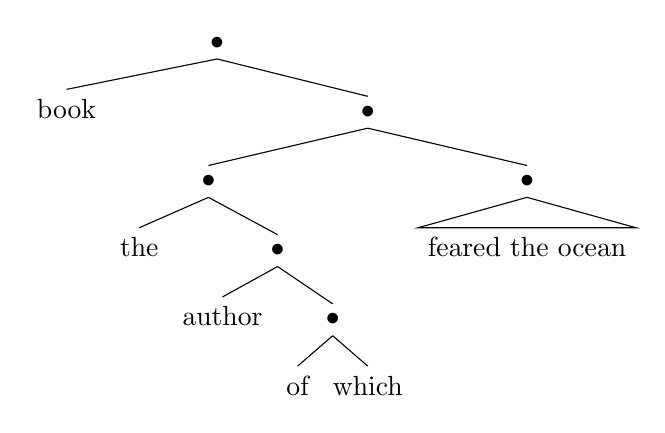
\begin{tikzpicture}[level distance=25]
      \Tree
      [.$\solp$ book [.$\solp$
      [.$\solp$ the [.$\solp$ author [.$\solp$ of which ] ] ]
      [.$\solp$ \edge[roof]; \node{feared the ocean}; ]
      ] ]
    \end{tikzpicture}
  }
  \only<3>{%
    \centering
    \vspace*{2em}
    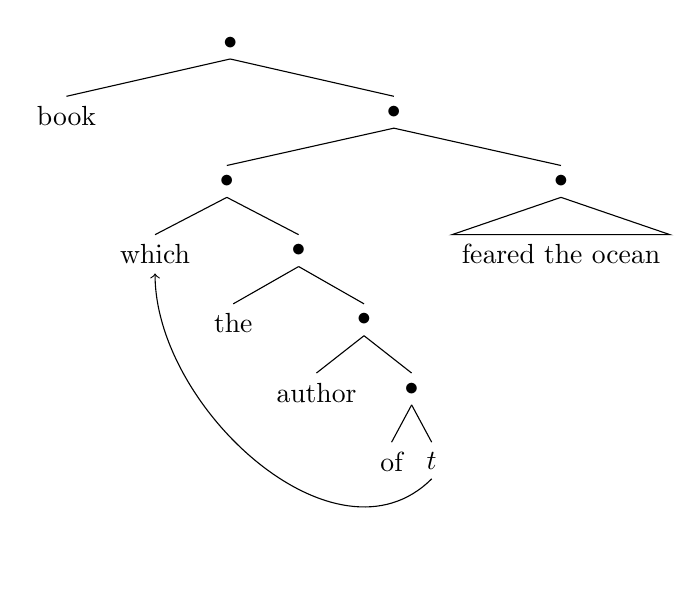
\begin{tikzpicture}[level distance=25]
      \tikzset{every tree node/.style={align=center,anchor=north}}  
      \Tree
      [.$\solp$ book [.$\solp$
      [.$\solp$ \node(which){which}; [.$\solp$ the
      [.$\solp$ author [.$\solp$ of \node(trace){$t$}; ] ] ] ]
      [.$\solp$ \edge[roof]; \node{feared the ocean}; ]
      ] ]
      \draw [->] (trace.south) to[out=-135,in=-90,looseness=1] (which.south);
    \end{tikzpicture}
  }  
  \only<4>{%
    \centering
    \vspace*{2em}
    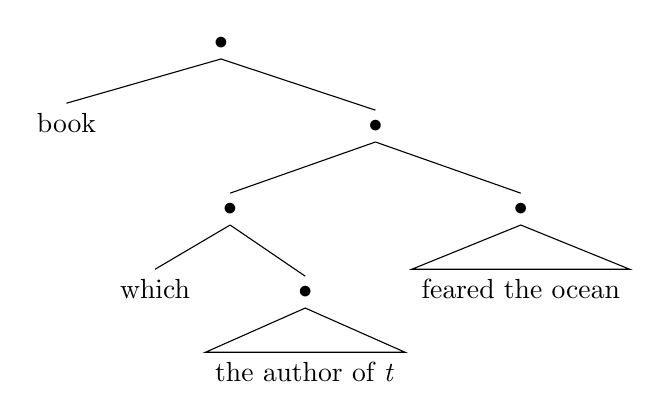
\begin{tikzpicture}
      \Tree
      [.$\solp$ book [.$\solp$
      [.{$\solp$}
      which [.$\solp$ \edge[roof]; \node{the author of \textit{t}};]]
      [.$\solp$ \edge[roof]; \node{feared the ocean};]
      ] ]
    \end{tikzpicture}
    \vspace*{1em}
    \begin{align*}
    &\text{which} \; : \; \llbracket np\hofs ( np\hobs ((n\sobs n)\sofs(np\sobs s)) ) \rrbracket \\
    &\text{which} =
      \lambda \text{tao}_{ee}.
      \lambda \text{fto}_{et}.
      \lambda \text{bk}_{et}.
      \lambda x_{e}.
      \text{bk}(x) \land \text{fto}(\text{tao}(x))
    \end{align*}
  }  
\end{frame}

\begin{frame}
  \frametitle{Why should we like NL$_{\lambda}$?}
  \centering
  \vspace*{2em}
  \begin{tikzpicture}[level distance=25]
    \Tree
    [.$\solp$ book [.$\solp$
    [.$\solp$ which [.$\holp$ $\lambda x$ [.$\solp$ the
    [.$\solp$ author [.$\solp$ of $x$ ] ] ] ] ]
    [.$\solp$ \edge[roof]; \node{feared the ocean}; ]
    ] ]
  \end{tikzpicture}
\end{frame}

\begin{frame}
  \begin{block}{Take-home message}
    NL$_\lambda$ gives us operational semantics for quantifier raising \`a la
    delimited continuations, without changing any other part of our type system.
  \end{block} 
\end{frame}

\begin{frame}
  \frametitle{Why should we like NL$_{CL}$?}
  \only<1>{%
    \centering
    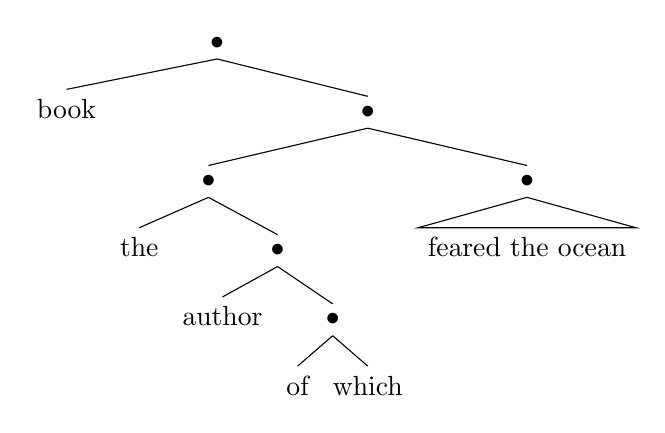
\begin{tikzpicture}[level distance=25]
      \Tree
      [.$\solp$ book [.$\solp$
      [.$\solp$ the [.$\solp$ author [.$\solp$ of which ] ] ]
      [.$\solp$ \edge[roof]; \node{feared the ocean}; ]
      ] ]
    \end{tikzpicture}
  }
  \only<2>{%
    \centering
    \vspace*{2em}
    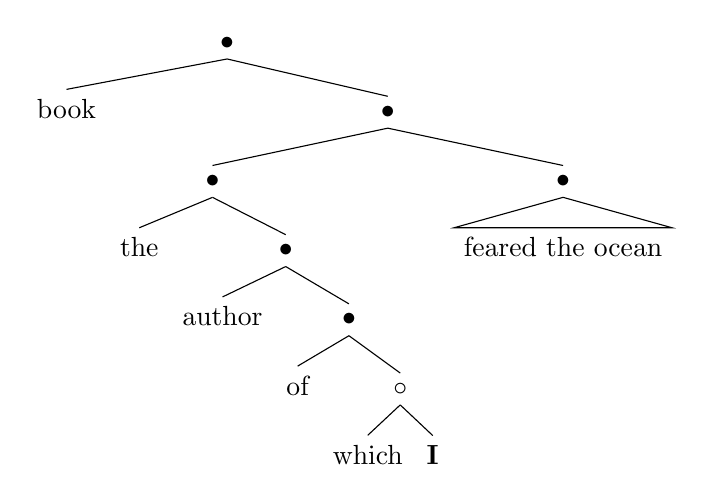
\begin{tikzpicture}[level distance=25]
      \Tree
      [.$\solp$ book [.$\solp$
      [.$\solp$ the [.$\solp$ author [.$\solp$ of [.$\holp$ which $\I$ ] ] ] ]
      [.$\solp$ \edge[roof]; \node{feared the ocean}; ]
      ] ]
    \end{tikzpicture}
  }
  \only<3>{%
    \centering
    \vspace*{2em}
    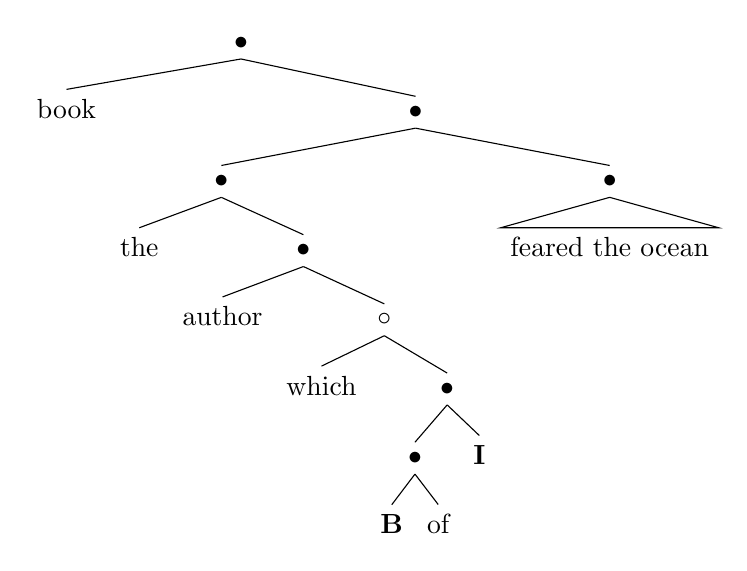
\begin{tikzpicture}[level distance=25]
      \Tree
      [.$\solp$ book [.$\solp$
      [.$\solp$ the [.$\solp$ author [.$\holp$ which
      [.$\solp$ [.$\solp$ $\B$ of ] $\I$ ] ] ] ]
      [.$\solp$ \edge[roof]; \node{feared the ocean}; ]
      ] ]
    \end{tikzpicture}
  }
  \only<4>{%
    \centering
    \vspace*{2em}
    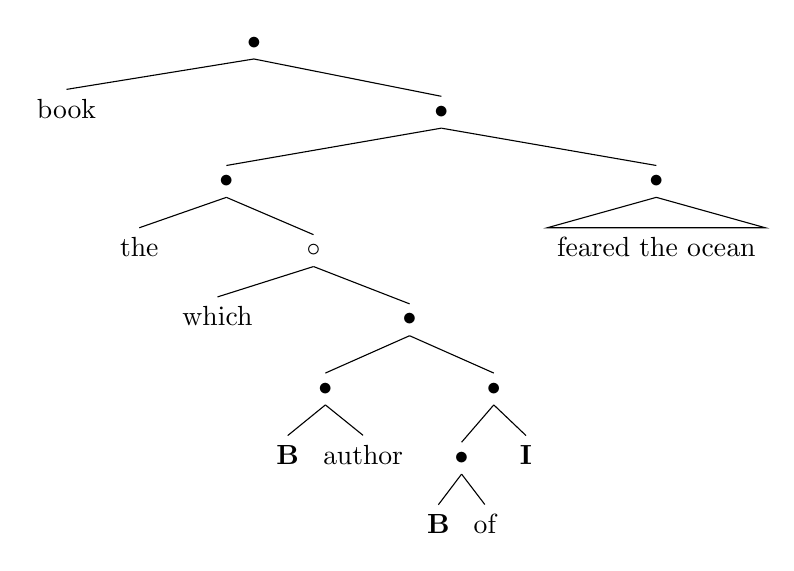
\begin{tikzpicture}[level distance=25]
      \Tree
      [.$\solp$ book [.$\solp$
      [.$\solp$ the [.$\holp$ which [.$\solp$  [.$\solp$ $\B$ author ]
      [.$\solp$ [.$\solp$ $\B$ of ] $\I$ ] ] ] ]
      [.$\solp$ \edge[roof]; \node{feared the ocean}; ]
      ] ]
    \end{tikzpicture}
  }
  \only<5>{%
    \centering
    \vspace*{2em}
    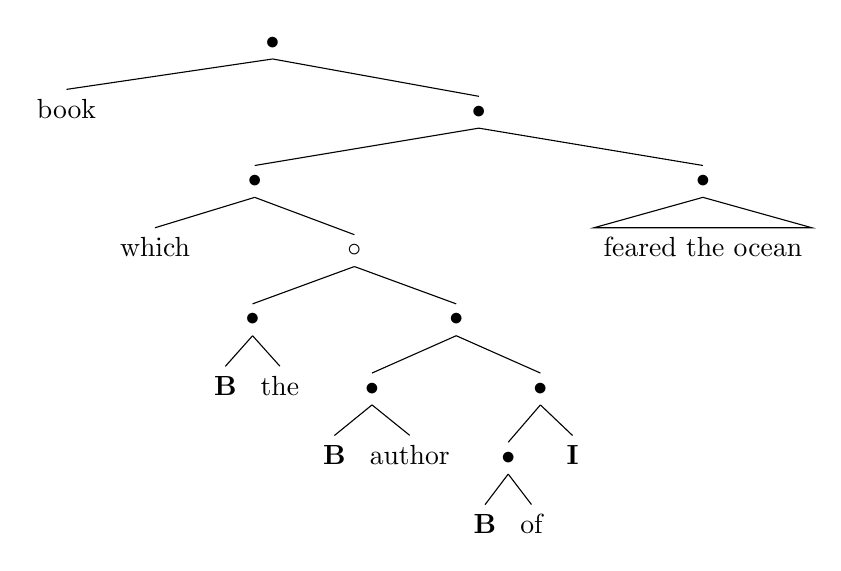
\begin{tikzpicture}[level distance=25]
      \Tree
      [.$\solp$ book [.$\solp$
      [.$\solp$ which
      [.$\holp$ [.$\solp$ $\B$ the ]
      [.$\solp$ [.$\solp$ $\B$ author ]
      [.$\solp$ [.$\solp$ $\B$ of ] $\I$ ] ] ] ]
      [.$\solp$ \edge[roof]; \node{feared the ocean}; ]
      ] ]
    \end{tikzpicture}
  }
\end{frame}

\begin{frame}
  \frametitle{Why should we like NL$_{CL}$?}
  \centering
  \vfill
  \(\!
  \begin{aligned}
    &\text{Structure}^+ \; \Gamma
    &&\coloneqq \ldots \mid \I \mid \B \mid \C
  \end{aligned}
  \)
  \vfill
  \begin{pfbox}
    \AXC{$\Gamma \fCenter \Delta$}
    \doubleLine
    \RightLabel{$\I$}
    \UIC{$\Gamma \holp \I \fCenter \Delta$}
  \end{pfbox}
  \vfill
  \begin{pfbox}
    \AXC{$\Gamma_1\prod(\Gamma_2\prod \Gamma_3)\fCenter \Delta$}
    \doubleLine\RightLabel{\B}
    \UIC{$\Gamma_2\prod((\B\prod \Gamma_1)\prod \Gamma_3)\fCenter \Delta$}
  \end{pfbox}%
  \begin{pfbox}
    \AXC{$(\Gamma_1\prod \Gamma_2)\prod \Gamma_3\fCenter \Delta$}
    \doubleLine\RightLabel{\C}
    \UIC{$\Gamma_1\prod((\C\prod \Gamma_2)\prod \Gamma_3)\fCenter \Delta$}
  \end{pfbox}
  \vfill
\end{frame}

\begin{frame}
  \frametitle{How do we parse with NL$_{CL}$?}
  \begin{block}{What do we change?}
    \begin{itemize}
    \item We restrict quantifier raising s.t.\ %
      \begin{itemize}
      \item \emph{only} quantifiers can be raised; and
      \item \emph{only} once.
      \end{itemize}
    \item We add focusing to eliminate spurious proofs.\footnote{%
        Following work by Michael Moortgat, Raffaella Bernardi and Richard Moot
        (2012) and Arno Bastenhof (2011).
      }
    \end{itemize}
  \end{block}
  \vspace{1em}
\end{frame}

\begin{frame}
  \frametitle{What does that look like?}
  \centering
  \vfill
  \(\!
  \begin{aligned}
    \text{Context}\;\Sigma\coloneqq\square\vsep\Sigma\prodl\Delta\vsep\Gamma\prodr\Sigma
  \end{aligned}
  \)
  \vfill
  \(\!
  \begin{aligned}
    \square   [\Gamma']&\mapsto \Gamma'\\
    (\Sigma\prodl\Gamma)[\Gamma']&\mapsto (\Sigma[\Gamma']\prod \Gamma)\\
    (\Gamma\prodr\Sigma)[\Gamma']&\mapsto (\Gamma\prod \Sigma[\Gamma'])
  \end{aligned}
  \qquad
  \begin{aligned}
    &\overline{\square}
    &&\mapsto \I\\
    \AXC{$$}
    &\overline{\Sigma\prodl\Gamma}
    &&\mapsto ((\C\prod \Sigma[\Gamma'])\prod \Gamma)\\
    &\overline{\Gamma\prodr\Sigma}
    &&\mapsto ((\B\prod \Gamma)\prod \Sigma[\Gamma'])
  \end{aligned}
  \)
  \vfill
  \begin{pfbox}
    \AXC{$\overline{\Sigma}\fCenter\struct{B}$}
    \AXC{$\struct{C}\fCenter\Delta$}
    \RightLabel{L$q$}
    \BIC{$\Sigma[\struct{C\himpl B}]\fCenter \Delta$}
  \end{pfbox}
  \begin{pfbox}
    \AXC{$\Sigma[\struct{A}]\fCenter\struct{B}$}
    \RightLabel{R$q$}
    \UIC{$\overline{\Sigma}\fCenter\struct{A\himpr B}$}
  \end{pfbox}
  \vfill
\end{frame}

\begin{frame}
  \begin{block}{Take-home message}
    If you had any qualms about the decidability and efficiency of proof search
    with NL$_\lambda$, let them go, at least for the remainder of this talk.
  \end{block}
\end{frame}

\begin{frame}
  \frametitle{Scope islands}
  \only<1>{%
    \centering
    \vfill
    \begin{block}{Example 2}
      ``Someone said $\langle \text{ Kurt wrote every book } \rangle$'' 
      \vfill
      \begin{gather*}
      \exists{x}.\PERSON(x)\wedge\SAY(x,\forall{y}.\BOOK(y)\supset\WROTE(\KURT,y))
      \end{gather*}
    \end{block}
    \vfill
  }
  \only<2>{%
    \centering
    \vspace{2em}
    \tikz[level distance=25]{%
      \Tree
      [.$\solp$ Someone [.$\solp$ said
      [.$\langle \cdot \rangle$
      [.$\solp$ \edge[roof]; \node{Kurt wrote every book}; ]
      ] ] ]
    }
    \vspace{1em}
    \begin{align*}
      &\text{said} : \; \llbracket (np \sobs s) \sofs \Diamond s \; \rrbracket \\
      &\text{said} = \ldots
    \end{align*}
  }
\end{frame}

\begin{frame}
  \frametitle{Not \emph{That} Diamond and Box}
  \vfill
  \begin{center}
    \(\!
    \begin{aligned}
      &\text{Formula}     &&\; A, B   &&\coloneqq \ldots\vsep\di A\vsep\sq A\\
      &\text{Structure}^+ &&\; \Gamma &&\coloneqq \ldots\vsep\langle \Gamma\rangle\\
      &\text{Structure}^- &&\; \Delta &&\coloneqq \ldots\vsep[\Delta]
    \end{aligned}
    \)
    \\[1\baselineskip]
    \begin{pfbox}
      \AXC{$\langle\struct{A}\rangle\fCenter \Delta$} \RightLabel{L$\di$}
      \UIC{$\struct{\di A}\fCenter \Delta$}
    \end{pfbox}
    \begin{pfbox}
      \AXC{$\Gamma\fCenter\struct{B}$} \RightLabel{R$\di$}
      \UIC{$\langle \Gamma\rangle\fCenter\struct{\di B}$}
    \end{pfbox}
    \\[1\baselineskip]
    \begin{pfbox}
      \AXC{$\struct{A}\fCenter \Delta$} \RightLabel{L$\di$}
      \UIC{$\struct{\sq A}\fCenter[\Delta]$}
    \end{pfbox}
    \begin{pfbox}
      \AXC{$\Gamma\fCenter[\struct{B}]$} \RightLabel{R$\sq$}
      \UIC{$\Gamma\fCenter\struct{\sq B}$}
    \end{pfbox}
    \\[1\baselineskip]
    \begin{pfbox}
      \AXC{$\Gamma\fCenter[\Delta]$} \doubleLine\RightLabel{Res$\sq\di$}
      \UIC{$\langle \Gamma\rangle\fCenter \Delta$}
    \end{pfbox}
  \end{center}
  \vfill 
\end{frame}

\begin{frame}
  \begin{block}{Take-home message}
  Things don't have to be difficult.   
  \end{block}
\end{frame}

\begin{frame}[label=indefinite-scope]
  \frametitle{Indefinite scope}
  \vfill
  \begin{block}{Example 3}
    ``Everyone said $\langle \text{ Kurt dedicated a book to Mary } \rangle$''
    \vfill
    \begin{gather*}
      \forall{x}.\PERSON(x)\supset\SAY(x,\exists{y}.\BOOK(y)
      \wedge\DEDICATE(\KURT,\MARY,y))
      \\
      \forall{x}.\PERSON(x)\supset\exists{y}.\BOOK(y)
      \wedge\SAY(x,\DEDICATE(\KURT,\MARY,y))
      \\
      \exists{y}.\BOOK(y)
      \wedge\forall{x}.\PERSON(x)\supset\SAY(x,\DEDICATE(\KURT,\MARY,y))
    \end{gather*}
  \end{block}
  \vfill
\end{frame}

\begin{frame}
  \begin{quote}
    ``Indefinites acquire their existential scope in a manner that does not
    involve movement and is essentially syntactically unconstrained.''\\
    \hfill --- Anna Szabolcsi, The Syntax of Scope
  \end{quote}
\end{frame}

\againframe{indefinite-scope}

\begin{frame}
  \centering
  (ramble about continuations)
\end{frame}

\begin{frame}
  \frametitle{Continuation Semantics}
  \begin{gather}
    \begin{aligned}
      &\text{some} : \; \llbracket \; np \sofs n \; \rrbracket
      \\
      &\text{some} \; (f, k) \; = \exists_{e} x. f(x) \land k(x)
    \end{aligned}
    \\[1\baselineskip]
    \AXC{$\overline{\Sigma}\fCenter\focus{np \hobs s}$}
    \AXC{$\focus{s}\fCenter\struct{s}$}
    \RightLabel{L$q$}
    \BIC{$\Sigma[\struct{s\hofs (np \hobs s)}]\fCenter \struct{s}$}
    \DisplayProof
    \\[1\baselineskip]
    \AXC{$
      \phantom{\langle}
      \text{Kurt dedicated \ldots}
      \phantom{\rangle}
      \fCenter\focus{\phantom{\di} s}$}
    \RightLabel{R$\di$}
    \UIC{$\langle\text{Kurt dedicated \ldots}\rangle\fCenter\focus{\di s}$}
    \AXC{$\focus{np \sobs s} \fCenter \text{everyone} \sobs \struct{s}$}
    \BIC{$
      \focus{(np \sobs s) \sofs \di s}\fCenter
      (\text{everyone} \sobs \struct{s})\sofs
      \langle\text{Kurt dedicated \ldots}\rangle$}
    \DisplayProof
 \end{gather}
\end{frame}

\againframe{indefinite-scope}

\begin{frame}[label=conclusion]
  \frametitle{What makes up a bunch?}
  \begin{itemize}
  \item[$\circ$] Display NL$_\lambda$
  \item[$\circ$] (Parasitic scope, delimited continuations)
  \item[$\circ$] Focusing and efficient proof search
  \item[$\circ$] Scope islands
  \item[$\circ$] Indefinite scope
  \end{itemize}
\end{frame}

\begin{frame}
  \centering
  \vfill
  \url{pepijn.kokke@gmail.com}
  \vfill
  \url{https://pepijnkokke.github.io/thesis.pdf}
  \vfill
\end{frame}

\begin{frame}
  \frametitle{A little bit of Haskell}
  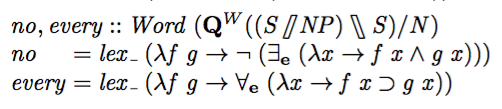
\includegraphics[width=\textwidth]{images/defs}
  \vfill
  \hspace*{-1em}%
  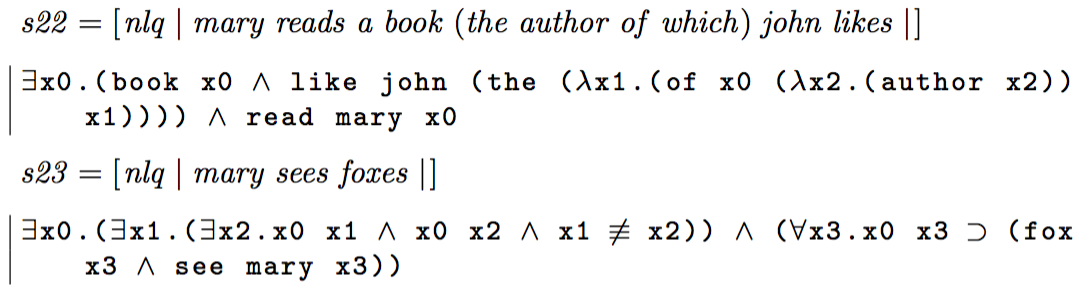
\includegraphics[width=\textwidth+2em]{images/ex2}
\end{frame}

\begin{frame}
  \frametitle{A little bit of Agda}
  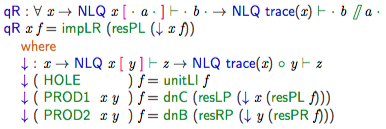
\includegraphics[width=\textwidth]{images/proof}
\end{frame}

\againframe{conclusion}

\appendix
\begin{frame}
  \Huge
  \centering
  Bonus Slides
\end{frame}

\begin{frame}
  \frametitle{What does focusing look like?}
  \centering
  \vfill
  \only<1>{%
    \[\!
      \begin{aligned}
        &\text{Pol}(np)        &&= {+}\\
        &\text{Pol}(n)         &&= {+}\\
        &\text{Pol}(s)         &&= {-}
      \end{aligned}
      \qquad
      \begin{aligned}
        &\text{Pol}(A \sobs B) &&= {-}\\
        &\text{Pol}(B \sofs A) &&= {-}\\ 
        \\
      \end{aligned}
    \]
    \vfill
    \[
      \text{Pos}(A) \iff \text{Pol}(A) = {+}
      \qquad
      \text{Neg}(A) \iff \text{Pol}(A) = {-}
    \]
  }
  \only<2>{%
    \[\!
    \text{if}\ \text{Pos}(\alpha)
    \left\lbrace
      \quad
      \begin{aligned}
        \\
        \AXC{}
        \RightLabel{Ax$^R$}
        \UIC{$\struct{\alpha}\fCenter\focus{\alpha}$}
        \DisplayProof
        \\[1\baselineskip]
      \end{aligned}
      \quad
      \normalcolor
      \middle\vert
      \normalcolor
      \quad
      \begin{aligned}
        \\
        \AXC{}
        \RightLabel{Ax$^L$}
        \UIC{$\focus{\alpha}\fCenter\struct{\alpha}$}
        \DisplayProof
        \\[1\baselineskip]
      \end{aligned}
      \quad
    \right\rbrace
    \normalcolor
    \text{if}\ \text{Neg}(\alpha)
    \]
    \[\!
    \text{if}\ \text{Pos}(A)
    \left\lbrace
      \quad
      \begin{aligned}
        \\
        \AXC{$\Gamma\fCenter\focus{A}$}
        \RightLabel{Foc$^R$}
        \UIC{$\Gamma\fCenter\struct{A}$}
        \DisplayProof
        \\[1\baselineskip]
        \AXC{$\struct{A}\fCenter \Delta$}
        \RightLabel{Unf$^L$}
        \UIC{$\focus{A}\fCenter\Delta$}
        \DisplayProof
        \\[1\baselineskip]
      \end{aligned}
      \quad
      \middle\vert
      \quad
      \begin{aligned}
        \\
        \AXC{$\focus{A}\fCenter\Delta$}
        \RightLabel{Foc$^L$}
        \UIC{$\struct{A}\fCenter \Delta$}
        \DisplayProof
        \\[1\baselineskip]
        \AXC{$\Gamma\fCenter\struct{A}$}
        \RightLabel{Unf$^R$}
        \UIC{$\Gamma\fCenter\focus{A}$}
        \DisplayProof
        \\[1\baselineskip]
      \end{aligned}
      \quad
    \right\rbrace
    \text{if}\ \text{Neg}(A)
    \]
  }
  \only<3>{%
    \begin{pfbox}
      \AXC{$\Gamma\fCenter\focus{A}$}
      \AXC{$\focus{B}\fCenter \Delta$}
      \RightLabel{L$\sobs$}
      \BIC{$\focus{A\sobs B}\fCenter \Gamma\sobs \Delta$}
    \end{pfbox}%
    \begin{pfbox}
      \AXC{$\Gamma\fCenter\focus{A}$}
      \AXC{$\focus{B}\fCenter \Delta$}
      \RightLabel{L$\sofs$}
      \BIC{$\focus{B\sofs A}\fCenter \Delta\sofs \Gamma$}
    \end{pfbox}
  }
  \vfill
\end{frame}


\begin{frame}
  \frametitle{Continuation Semantics}
  \centering
  \(\!
  s^*  \mapsto \t,
  \qquad
  n^*  \mapsto \e\t,
  \qquad
  np^* \mapsto \e,
  \qquad
  \ldots 
  \)
  \vfill
  \only<1>{%
  \(\!
  \begin{aligned}
    &\tr{\alpha}^+ &&\mapsto
    \begin{cases}
      \phantom{((}\alpha^*
      &
      \mbox{if Pos}(\alpha)
      \\
      ((\alpha^*)^R)^R
      &
      \mbox{if Neg}(\alpha)
    \end{cases}
    \\
    &\tr{A\impr B}^+ &&\mapsto (\tr{A}^+\times\tr{B}^-)^R \\
    &\tr{B\impl A}^+ &&\mapsto (\tr{B}^-\times\tr{A}^+)^R \\
    &\tr{\di A}^+ &&\mapsto \tr{A}^++ \\
    &\tr{\sq A}^+ &&\mapsto (\tr{A}^++)^R \\
  \end{aligned}
  \)
  }
  \only<2>{
    \(\!
    \begin{aligned}
      &\tr{\alpha}^-   &&\mapsto (\alpha^*)^R \\
      &\tr{A\impr B}^- &&\mapsto \tr{A}^+\times\tr{B}^- \\
      &\tr{B\impl A}^- &&\mapsto \tr{B}^-\times\tr{A}^+ \\
      &\tr{\di A}^-    &&\mapsto (\tr{A}^++)^R \\
      &\tr{\sq A}^-    &&\mapsto \tr{A}^++ \\
    \end{aligned}
  \)}
  \only<3>{%
    \(\!
    \begin{aligned}
      &\tr{\Gamma\fCenter\Delta} &&\mapsto \tr{\Gamma}\fCenter\tr{\Delta} \\
      &\tr{\focus{A}\fCenter\Delta} &&\mapsto \tr{\Delta}\fCenter\tr{A}^- \\
      &\tr{\Gamma\fCenter\focus{A}} &&\mapsto \tr{\Gamma}\fCenter\tr{A}^+
    \end{aligned}
    \)
  }
  \vfill
  \(\!
  (\text{where} \; A^R \coloneqq A \to \t)
  \)
\end{frame}

\bibliographystyle{apalike}
\bibliography{main}

\end{document}
